\documentclass[a4paper,11pt,notitlepage]{report}

\usepackage[utf8]{inputenc}
\usepackage{amsmath}
\usepackage{listings}
\usepackage[hidelinks]{hyperref}
\usepackage{catoptions}
\usepackage[left=0.8in, right=0.8in, top=0.8in, bottom=0.8in]{geometry}
\usepackage{color}
\usepackage{soul}
\usepackage{float}
\usepackage{framed}
\usepackage[sc]{mathpazo}
\linespread{1.20}         % Palatino needs more leading (space between lines)
\usepackage[T1]{fontenc}
\usepackage{microtype}
\usepackage{enumerate}
\usepackage{courier}
\usepackage{graphicx}
\usepackage{enumitem}
\usepackage{lipsum}
\usepackage{tikz}
\usepackage{caption}
\usepackage{subcaption}
\usepackage{verbatim}
\usetikzlibrary{shapes,arrows}

\graphicspath{ {./Images/} }

\pdfinfo{
  /Title    (Building Serious Games - Design4Health)
  /Author   (Ralf Nieuwenhuizen, David Prihoda, Ismini Psuxoula, Arnold Schutter, Shen Shuheng)
  /Creator  (Ralf Nieuwenhuizen, David Prihoda, Ismini Psuxoula, Arnold Schutter, Shen Shuheng)
  /Producer (Ralf Nieuwenhuizen, David Prihoda, Ismini Psuxoula, Arnold Schutter, Shen Shuheng)
  /Subject  (Building Serious Games)
}

% Settings for hyperref package (e.g. wat \autoref en \nameref moeten doen)
\hypersetup{
  colorlinks  = false,
  linkcolor   = [rgb]{0.1,0.1,0.5},
  citecolor   = [rgb]{0.5,0.1,0.1},
  filecolor   = [rgb]{0.1,0.5,0.5},
  urlcolor    = [rgb]{0.1,0.1,0.7}
}

\newcommand{\todo}[1] {\hl{#1}}
\setlength{\parindent}{0cm}

\begin{document}

% Define block styles
\tikzstyle{block} = [rectangle, draw, fill=white!20, 
    text width=7em, text centered, rounded corners, minimum height=4em]
\tikzstyle{blockSmall} = [rectangle, draw, fill=white!20, 
    text width=4em, text centered, rounded corners, minimum height=3em]
\tikzstyle{line} = [draw, -latex']
		
\begin{center}
\vskip 1cm
{\Huge Design4Health \vskip 2mm}
{\Large IN4302TU -- Building Serious Games \vskip 1cm}
{\Huge Synopsis \& Responsibilities \vskip 1cm}

\begin{tabular}{ l l }
\textbf{Ralf Nieuwenhuizen} & ($4080408$) \\
\textbf{David Prihoda} & ($4405951$) \\
\textbf{Ismini Psychoula} & ($4411285$) \\ 
\textbf{Arnold Schutter} & ($4260724$) \\ 
\textbf{Shuheng Shen} & ($4298225$)
\end{tabular} 

\end{center}

%\newpage
%\tableofcontents
%\newpage

\chapter{Team}

The team consists of $5$ members, all having an own main responsibility. These will be explained below.

\section{Responsibilities}

\begin{itemize}
	\item Ralf Nieuwenhuizen: Communication
	\item David Prihoda: Lead Artist
	\item Ismini Psychoula: Lead programmer
	\item Arnold Schutter: Lead Game Design
	\item Shuheng Shen: Lead Testing
\end{itemize}

\subsection{Communication}
The communicator is responsible for the timely communication with external parties and the teacher including weekly updates. 

\subsection{Lead Artist}
The lead artist is responsible for gameplay and graphics. Gameplay (fun) should continuously be checked and the graphics should be made according to a graphical design plan. The lead artist is responsible for this plan and prioritizing tasks.

\subsection{Lead Programmer}
The lead programmer is responsible for keeping the overview of the software (architecture) and for quality. The lead programmer prioritizes the milestones for the software and checks for the quality and coherence. When deliverables are not satisfactory, the lead programmer is allowed to let deliverables be rectified.

\subsection{Lead Game Design}
The lead game designer is responsible for the overall planning and the coherence between the software and the game design. 

\subsection{Lead Testing}
The lead tester is responsible for weekly testing the deliverables for appearance, errors/bugs, gameplay quality and coherence. The Lead Tester prioritizes the tasks to be improved together with the Lead Programmer. 

\chapter{Planning}
The group will work with a scrum-based system, where the tuesday meetings will be used for planning, and the friday sessions for evaluation.

\section{Meetings}
Our weekly meetings are at:
\begin{itemize}
	\item Monday $08.45$ - $10.30$
	\item Tuesday $12.30$ - $16.30$
	\item Thursday $13.45$ - $15.30$
	\item Friday $13.45$ - $16.30$
\end{itemize}

\section{Schedules}
See the figures below for an initial planning (figure~\ref{fig:planning}) and a list of tasks (table~\ref{tab:todolist}).
Future tasks will be tracked using the github issue tracker.
Since we are using the issue tracker on github, we can use our commit messages to set the issue status to fixed/closed, simply by putting [closes \#7] or [fixes \#6] in the commit message. If a commit doesn't fix or closes anything, the commit message has to contain the issue number, i.e. [\#6], to be able to keep track of what feature it belongs to.

\begin{figure}[H]
	\centering
		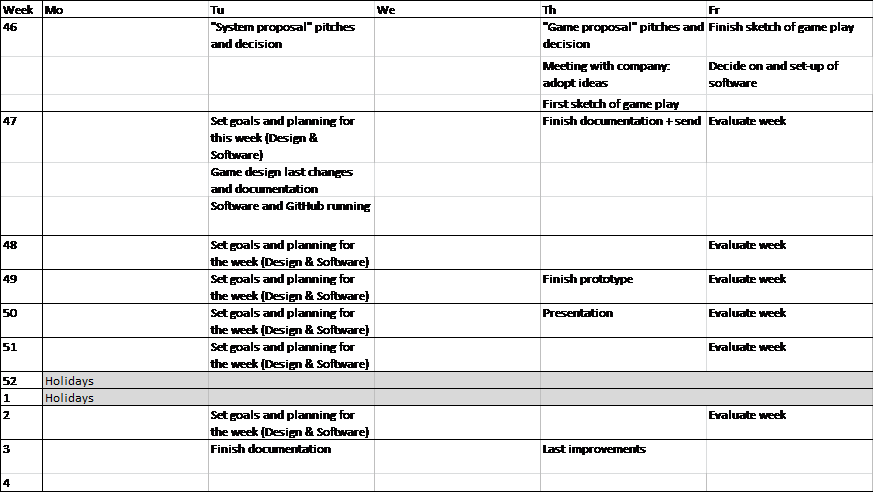
\includegraphics[width=\textwidth]{Images/PlanningSmall.png}
	\caption{Planning}
	\label{fig:planning}
\end{figure}

\begin{table}
\begin{tabular*}{1.075\textwidth}{ | l | l | l | l | l | }
\hline
	Week & Start date & Own Milestone & Action holder & Deadline \\ \hline
	46 & 10-11-2014 & Proposal synopsis & Arnold & 13-11-2014 \\ \hline
	 &  & Hand in game synopsis to Prof & Ralf & 14-11-2014 \\ \hline
	 &  & Set up GitHub & Ralf & 14-11-2014 \\ \hline
	47 & 17-11-2014 & Static prototype presentation & David and Shuheng & 18-11-2014 \\ \hline
	 &  & Software pres and cons overview & Ismini & 18-11-2014 \\ \hline
	 &  & Decision on software platform & All & 18-11-2014 \\ \hline
	 &  & Finish test accelerometer posibilities & Ismini & 20-11-2014 \\ \hline
	 &  & Hand in game design document & Ralf & 21-11-2014 \\ \hline
	48 & 24-11-2014 &  &  &  \\ \hline
	 &  &  &  &  \\ \hline
	49 & 1-12-2014 & Hand in game prototype & Ralf & 5-12-2014 \\ \hline
	 &  &  &  &  \\ \hline
	50 & 8-12-2014 & Finish and prepare presentation (2 persons!) & Ralf (you can delegate) & 9-12-2014 \\ \hline
	 &  &  &  &  \\ \hline
	51 & 15-12-2014 & Hand in game prototype Beta & Ralf & 19-12-2014 \\ \hline
	 &  & Invite company for final presentation & Ralf & 19-12-2014 \\ \hline
	52 & 22-12-2014 &  &  &  \\ \hline
	 &  &  &  &  \\ \hline
	1 & 29-12-2014 &  &  &  \\ \hline
	 &  &  &  &  \\ \hline
	2 & 5-1-2015 &  &  &  \\ \hline
	 &  &  &  &  \\ \hline
	3 & 12-1-2015 & Hand in game prototype \& documentation & Ralf & 16-1-2015 \\ \hline
	 &  &  &  &  \\ \hline
	4 & 19-1-2015 & Finish and prepare presentation (2 persons!) & Ralf (you can delegate) & 19-1-2015 \\ \hline
\end{tabular*}	
	\caption{Initial todo-list}
	\label{tab:todolist}
\end{table}

\chapter{Game design}
As can be seen from the planning in the previous section, a game will be created in a couple of stages. In this section there shall be some explanation on the commissioner's assignment, the outline of the envisioned game, and how this will be realised.

\section{Assignment}
The official game description does not contain specific requirements. The purpose of the game is to motivate or help people to do exercises to get fit and healthy. Exercises are possibly but not necessarily provided by a physiotherapist. 

\section{Design concept}
The concept of the design is an engaging game for which the user needs to perform exercises in order to make progress in the game. By executing more and more exercises the user has more possibilities in the game and new challenges will become available. 

\subsection{Game Story}
The game starts with a story. 
\\ 
\\
\textit{2542 AD. Your uncle was one of the first people to buy land in an unknown planet and decided to turn it into a farm to facilitate the earth’s growing needs of foods. As years went by the farm became very profitable and produced the most sought out products. You were very surprised when you received a mail saying that your uncle had left you the farm years ago but you only learned of it now. After so many years the fields are unused and empty. Will you be able to salvage the farm? Spend your money wisely to grow the company and unlock new possibilities by doing the exercises.}

\subsection{Gameplay}
The game is about a farm and the user is the farmer. By growing crops and keeping lifestock the farmer can grow the company and make money. However, crops and lifestock are only available when certain skills are available. To show certain skills, the farmer has to execute exercises in real-life. An exercise is specific for each crop or lifestock. For example, the skill for picking apples has to be shown before the appletrees can be bought. 

After showing a certain skill, the belonging crop or lifestock is unlocked so it can be bought. However, things can only be bought when the farmer has sufficient money, space and energy. The amount of energy represents the time and energy of the farmer during one day. This amount is fixed at the beginning, but can be increasing by becoming more active, or by hiring partners or buying hulpful equipment. The amount of space around the farm is fixed throughout the duration of the game. While the game progresses, some old crops or lifestock might be sold to free space for new options.

The farmer can make money by selling products on the market. Crops should be harvested first, this is done by executing the corresponding exercises for the specific crop. Gaining products from life stock such as milk from the cow also requires the execution of exercises before it is available to be sold. Preparing and selling products on the market also takes energy.

During the game, the farmer is allowed to buy machinery or equipment to enlarge the available amount of energy during the day. The extra energy is however only available when an exercise, corresponding to the specific item, is performed during the day. For example, when a pump is bought and this gives $10$ extra energy, the farmer should do the pumping exercise to gain the $10$ extra energy for that day. 

Every now and then the farmer receives a special order or task. This can be for example the delivery of specific crops or products during the period. When the farmer completes these tasks, the game will advance to the next level. A new level introduces new crops, lifestock and equipment.

When the exercises are performed sensors are used to measure the movements along with sounds and visualizations to increase the interactivity of the game and make the experience fun.

\section{Advanced Exercises}
Exercises can specifically be designed by physiotherapists for certain phsyiotherapeutic problems, so these exercises are very useful for certain users. By having these users execute the exercises, that apply to their injury, in the game, they follow a special training program without even noticing.  

\section{Design construct}
A diagram of the different components of the game is shown in figure~\ref{fig:gameconcept}.

\begin{figure}[h]
	\centering
		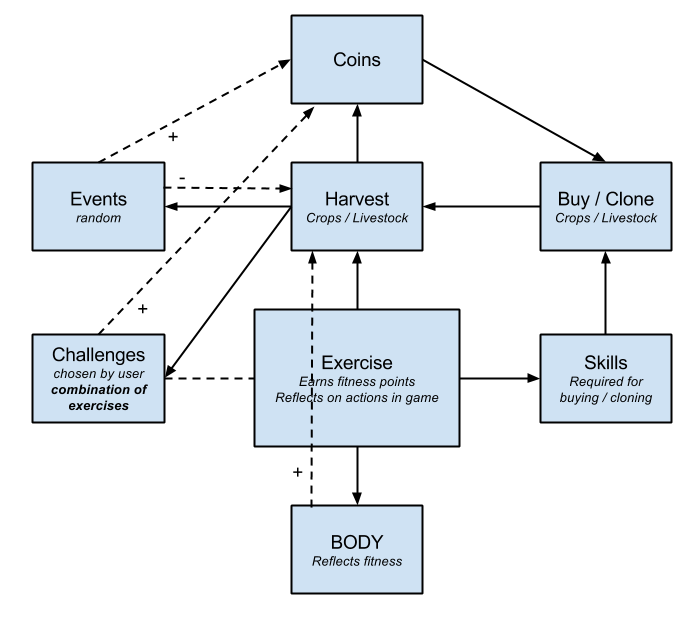
\includegraphics[width=0.80\textwidth]{Images/gameconcept.png}
	\caption{Component diagram of the game}
	\label{fig:gameconcept}
\end{figure}

\section{Fulfilling requirements}
The envisioned design will fulfill the requirement of being an engaging, activating game. This is all meant to activate people while doing an activity they love, gaming. As there are no real age requirements, an age group will be set as soon as we determine how complex the game will be. Adding features to the farm will make the game more appropriate for older people (think of people over $12$ years), and keeping it simple will keep the target age group a little younger (more like $8$-$14$ years). The game will be serious, as there is a clear purpose behind it of activating people, and it will be fun, as is proven by previous games in which you build up your own world, and have to show dedication to keep it up and running.

\section{Prototype}
To get a feeling of how the final release of the game will be and to test whether the idea is really as engaging as it sounded at first, there will be some prototyping in the early stages of the project.

\subsection{Designing the game}
Before starting on developing the actual software, there will be sketches for all screens of the game, to create a clickable static prototype. This will be presented to the group, and after that final decisions are made on the design.

\subsection{First playable}
The first playable will be a small version of the final game. It will not be as complete, but the vital functions will be there, for example the farm, some sort of crop, the money, place and energy, and some livestock. There will be some user tests and the progress will be reported to the commissioners.

\subsection{Resources}
To get from a paper prototype to a full up and running game some resources will be needed. Because it will be a smartphone application, no external sensors will be needed. Plenty of open source software is available to fulfill our needs. The only cost we will have is the Android Developer registration fee which is \$25
\subsubsection{Hardware}
The only requirement for someone to play our game will be that he owns a smartphone. Research about the sensors on each phone we can use will be done. Most likely these will include the accelerometer, GPS, and microphone.
\subsubsection{Software}
The game will be developed for Android mobile phones, using open source software. 
We will most likely go for HTML5 supported by javascript, eventually with supporting libraries. The HTML5 can be converted to a native app by using PhoneGap (\url{http://phonegap.com/}). This also gives us the option to convert to other mobile platforms, like iOS and Windows (Phone)


%\bibliography{synopsis}
%\bibliographystyle{plain}

\end{document}
